% !TEX root = LF-IMAPol.tex

\chapter{Preliminary linguistic notions}\label{chap:preliminaryNotions}

The description of lexical functions requires a preliminary set of linguistic notions that we need to make use of throughout the present volume. This chapter offers the reader a concise presentation of those notions, which are grouped into three classes: lexical notions (\sectref{sec:lexicalNotions}), semantic notions (\sectref{sec:semanticNotions}) and syntactic notions (\sectref{sec:syntacticNotions}).

What follows is a series of definitions\index[notion]{definition!\tld\ of notions} supplied with explanations and illustrations. Two types of definitions are used: analytic and enumerative definitions.

\phantomsection\label{txt:lexicographicDefinition}\notion{Analytic definitions}\index[notion]{definition!analytic \tld} constitute the basic type; they follow the Aristotelian definition pattern \textit{per genus proximum et differentia specifica} (`by next kind and specific differences') -- e.g., definitions for \textit{lexeme} and \textit{idiom} below. These definitions are of almost the same structure as lexicographic definitions\index[notion]{definition!lexicographic \tld|emph} described in \textcite{MelcukPolguere2018}.\footnote{For examples of actual lexicographic definitions, see the definitions of \textsc{snow}\tsub{(N)} in \chapref{chap:paraLFs} (\sectref{sec:LFapparenteesSynAnti}, p.\thinspace\pageref{ldef:defSNOW-n}), \textsc{debt} in \chapref{chap:syntLFs} (\sectref{sec:verbeReal}, p.\thinspace\pageref{ldef:defDEBT}) and \textsc{anger}\tsub{(N)} in the Appendix (p.\thinspace\pageref{def:ANGER-n}).} The first component of the definition is the \notion{central} (or \notion{generic}) \notion{component}\index[notion]{component of a definition!central \tld|emph}\index[notion]{definition!central component of a \tld|emph}, and it corresponds to the Aristotelian \textit{genus proximum}. It is followed by a series of \notion{peripheral components}\index[notion]{component of a definition!peripheral \tld|emph}\index[notion]{definition!peripheral component of a \tld|emph}, which correspond to \textit{differentia specifica}; each peripheral component is introduced by a bullet (``{\footnotesize $\bullet$}'').

Marginally, \notion{enumerative definitions}\index[notion]{definition!enumerative \tld} are also used. They are structured as disjunctive lists of previously defined notions -- e.g., the definition for \notion{lexical unit} [=~lexeme or idiom] below (p.\thinspace\pageref{def:lexicalUnit}).

\section{Lexical notions}\label{sec:lexicalNotions}

Lexical functions, as their name suggests, are primarily about the lexicon\index[notion]{lexicon} and the units that constitute it, i.e., words and phraseological expressions. Therefore, we begin with linguistic notions related to words, on the understanding that the word \textit{word} is both too ambiguous and vague to belong to linguistic (in particular, lexicological) terminology. Let us start with the notion of \notion{lexeme}\index[notion]{lexeme|emph}.

\phantomsection\label{def:lexeme}\begin{notiondefinition}{lexeme}
A \notion{lexeme} is a set of wordforms\index[notion]{wordform} and analytic-form phrases\index[notion]{analytic-form phrase} such that \\*
\setlength{\tabcolsep}{.5pt}\begin{tabular}{ p{0.2cm} >{\raggedright\arraybackslash}p{10.5cm} }
\SpecDiff & their semantic, syntactic and morphological differences can be fully described in terms of inflectional significations.\\[3pt]
\end{tabular}

\noindent
\remark{Example.}The lexeme \textsc{amaze} = \{\thinspace\textit{amaze}, \textit{amazes}, \textit{amazed}, \textit{amazing}, \textit{have amazed}, \textit{will amaze}, \textit{am amazed}, \textit{being amazed}, \textit{will have amazed}, ...\thinspace\}.
\end{notiondefinition}\index[notion]{inflection}

A lexeme name is printed in \textsc{small capitals}, when needed accompanied by its part of speech\index[notion]{part of speech [PoS]} and \notion{lexicographic number}\index[notion]{lexicographic number|emph} (in case of polysemy\index[notion]{polysemy}\slashs{}homonymy\index[notion]{homonymy}) -- e.g., \lu{picture}{(N)}{}{I.1} `image', \lu{picture}{(N)}{}{I.2} `movie', \lu{picture}{(N)}{}{II} `mental representation'.\footnote{On lexicographic numbers used in Explanatory Combinatorial Lexicology, see \textcite[Ch.~13, Sec.~3.1]{Melcuk2013c-e}.}\index[notion]{Explanatory Combinatorial!\tld\ Lexicology}\index[notion]{lexicology!Explanatory Combinatorial \tld} Lexicographic numbers used in this book are not borrowed from a particular lexicographic description, unless specified otherwise. They are, so to speak, conventional and serve only to distinguish word senses.

Lexemes are one of the two types of lexical units, the second one being idioms (see below). Lexemes are the primary type, as will be shown shortly. The above definition relies on the morphological\index[notion]{morphology} notions of \notion{wordform}\index[notion]{wordform} and \notion{inflection}\index[notion]{inflection}, which have to be taken for granted here. A lexeme can be conceived of as a generalization over a set of wordforms and analytic-form phrases that all carry the same lexical meaning in their signified\index[notion]{signified}, while being related by shared signifiers\index[notion]{signifier}.

The next notion to be defined is that of (lexemic) \notion{phraseme}\index[notion]{phraseme|emph}. It is a core preliminary notion for two reasons:

\begin{enumerate}

\item Idioms\index[notion]{idiom} (e.g., \idiom{\textsc{pull the plug}}) -- the second type of lexical units that we need to define -- are a particular class of phrasemes.

\item Lexical functions are especially relevant for the description of collocations\index[notion]{collocation} (e.g., \textit{wide awake} or \textit{pay attention}), which are also a particular case of phrasemes (\chapref{chap:NotionLF}, \sectref{sec:classeFLSyntagmatiques}, p.\thinspace\pageref{def:collocation}).

\end{enumerate}

In the following definition, the term \notion{Speaker}\index[notion]{Speaker, the|emph}, written with a capital \textit{S}, refers to the producer of the utterance under consideration (as opposed to a \textit{speaker} of a language). The corresponding receiver of the utterance is referred to as the \notion{Addressee}\index[notion]{Addressee|emph}, with a capital \textit{A}.

\phantomsection\label{def:phraseme}\begin{notiondefinition}{(lexemic) phraseme}
A (lexemic) \notion{phraseme} is a complex lexemic expression such that \\*
\setlength{\tabcolsep}{.5pt}\begin{tabular}{ p{0.2cm} >{\raggedright\arraybackslash}p{10.5cm} }
\SpecDiff & the selection of at least one of its lexemes by the Speaker is not free -- i.e., it is constrained by another lexeme of this expression. \\[3pt]
\end{tabular}

\noindent
\remark{Example.}The phraseme \textit{wide awake}, where the Speaker's choice of \textit{wide} to express `fully' is constrained by the adjective \textit{awake}; \textit{wide awake} can be contrasted with the non-idiomaticity of *\textit{wide dressed} `fully dressed', *\textit{wide ready} `fully ready', *\textit{wide known} `fully known' (cf. idiomatic phrase \textit{widely known}), etc.
\end{notiondefinition}

The presence of phrasemes is overwhelming in natural languages; the set of all phrasemes of a given natural language is called its \notion{phraseology}\index[notion]{phraseology}. In this volume, we concentrate on lexemic phrasemes\index[notion]{phraseme!lexemic \tld} (in particular, idioms and collocations) and disregard other families of phrasemes, such as syntactic\index[notion]{phraseme!syntactic \tld} and morphemic phrasemes\index[notion]{phraseme!morphemic \tld} \parencites[Ch.~16]{Melcuk2015a-e}{Melcuk2021b}{Melcuk2023a}. Therefore, the modifier \textit{lexemic} will be omitted.

Equipped with the definition of phraseme, we can define the second type of lexical unit (along with lexemes): \notion{idiom}\index[notion]{idiom|emph}.

\phantomsection\label{def:idiom}\begin{notiondefinition}{idiom}
An \notion{idiom} is a phraseme such that \\*
\setlength{\tabcolsep}{.5pt}\begin{tabular}{ p{0.2cm} >{\raggedright\arraybackslash}p{10.5cm} }
\SpecDiff & it is semantically non-compositional. \\[3pt]
\end{tabular}

\noindent
\remark{Example.}The idiom \idiom{\textsc{green thumb}} `great ability to take care of plants'.
\end{notiondefinition}

An idiom's name is enclosed between two top corners: \idiom{\textsc{green thumb}}, $\ulcorner$\textsc{rock the boat}$\urcorner$, \idiom{\textsc{by and large}}, ...

In the above definition, the phrase \textit{is semantically non-compositional}\index[notion]{compositionality, semantic|emph}\index[notion]{semantic!\tld\ (non-)compositionality|emph} refers to the fact that the meaning of an idiom is not a regular linguistic union\index[notion]{linguistic union \lfgp{operation}} of the meanings of its lexical components,\footnote{On the operation of linguistic union, see \chapref{chap:NotionLF}, \sectref{sec:LFcombination}, p.\thinspace\pageref{sec:LFcombination}.} so that a lexicographic definition\index[notion]{definition!lexicographic \tld} is required to describe an idiom's meaning. Three types of idioms are distinguished as regards their meaning: strong, semi- and weak idioms.

\begin{itemize}

\item A \notion{strong idiom}\index[notion]{idiom!strong \tld|emph} has a meaning that does not contain the meaning of any of its components -- e.g., \idiom{\textsc{shoot the breeze}} `talk leisurely'.

\item A \notion{semi-idiom}\index[notion]{idiom!semi-\tld|emph} has a meaning that contains the meanings of some of its lexical components -- e.g., \idiom{\textsc{morning sickness}} `nauseous feeling experienced by a pregnant woman typically in the \emph{morning}'.

\item A \notion{weak idiom}\index[notion]{idiom!weak \tld|emph} has a meaning that contains the meanings of all its lexical components plus additional semantic material -- e.g., \idiom{\textsc{bacon and eggs}} `dish made of fried \emph{eggs and} fried \emph{bacon}'.

\end{itemize}

\begin{soundboxnotitle}

Semantic non-compositionality is often mistaken for opacity\index[notion]{opacity of a phraseme} or transparency\index[notion]{transparency of a phraseme}, which are relevant to the perspective of the Addressee\index[notion]{Addressee}, i.e., to understanding\index[notion]{understanding by the Addressee} of speech. Non-compositionality, however, is about the Speaker, who has to produce the idiom out of the semantic content the Speaker seeks to express. Idioms, especially semi- and weak idioms, are often easily interpretable by Addressees who do not know them. Even strong idioms can be based on metaphors that are quite transparent, at least in the contexts of use; such is the case of \idiom{\textsc{have one's hands full}} `be very busy', \idiom{\textsc{in a nutshell}} `concisely', etc. The semantic \mbox{(non-)}compositionality of an expression should therefore be estimated \emph{strictly} by contrasting its meaning as a whole with that of the lexical (and grammatical) material it is formally made up from, without recourse to hypothetical understanding processes.

(Non-)compositionality is relevant in the perspective of speech production\index[notion]{speech!\tld\ production}, while transparency is strictly about speech understanding\index[notion]{speech!\tld\ understanding}. Since this book takes the Meaning-Text approach\index[notion]{Meaning-Text!\tld\ approach}, it is exclusively \mbox{(non-)}compositionality that we consider in order to characterize idioms.

\end{soundboxnotitle}

Now that both notions of lexeme and idiom have been defined and clarified, we can offer an enumerative definition of \notion{lexical unit}\index[notion]{lexical unit|emph}.

\phantomsection\label{def:lexicalUnit}\begin{notiondefinition}{lexical unit}
A \notion{lexical unit} is a lexeme or an idiom.
\end{notiondefinition}

Note that there is another, marginal type of lexical unit, which we do not mention in the above definition in order to simplify the presentation: \notion{compounding elements}\index[notion]{compounding!\tld\ element}, also called \textit{combining forms} \parencite{Prcic2005,Prcic2008} -- e.g., \textsc{anthropo-} (in \textit{anthropomorphic}, ...), \textsc{neuro-} (\textit{neuroscience}, ...), or \textsc{-phile} (\textit{francophile}, ...), \mbox{\textsc{-phobia}} (\textit{arachnophobia}, ...). They are defective lexemes, in the sense that they cannot be used independently: they function only in compounding.

A lexical unit is the unit of the linguistic description of a language's lexicon\index[notion]{lexicon}. To put it differently, it is a unit of lexicographic description\index[notion]{lexicography}. That is, a lexical unit is described by a \notion{lexical entry}\index[notion]{lexical entry|emph}, of which it is the \notion{headword}\index[notion]{headword of a lexical entry}\index[notion]{lexical entry!headword of a \tld}.

In conformity with the principles of the description of linguistic signs\index[notion]{linguistic sign|emph} \parencite[Ch.~11, Sec.~2]{Melcuk2013c-e}, the lexical entry for a given lexical unit L accounts for three major components of L:\footnote{Strictly speaking, what follows is a characterization of the lexical entry of a lexeme. We do not indicate the particularities of the lexical entries of idioms, which are formally more complex.}

\begin{enumerate}

\item L's \notion{signified}\index[notion]{signified!\tld\ of a lexical unit} -- described in the \notion{semantic zone}\index[notion]{lexical entry!semantic zone of a \tld|emph}\index[notion]{semantic!\tld\ zone of a lexical entry|emph}\index[notion]{zone of a lexical entry!semantic \tld|emph} of the lexical entry, which is centered around L's lexicographic definition\index[notion]{definition!lexicographic \tld}; other possible elements of this zone are, for instance, \notion{lexical connotations}\index[notion]{connotation, lexical} \parencite{IordanskajaMelcuk2009a}.

\item L's \notion{signifier}\index[notion]{signifier!\tld\ of a lexical unit} -- described in the \notion{phonological\slashs graphematic zone}\index[notion]{lexical entry!phonological\slashs graphematic zone of a \tld|emph}\index[notion]{zone of a lexical entry!phonological\slashs graphematic \tld|emph} of the entry.

\item L's \notion{syntactics}\index[notion]{syntactics}, or \notion{restricted cooccurrence}\index[notion]{cooccurrence, restricted!\tld\ of a lexical unit|emph}\index[notion]{lexical unit!restricted cooccurrence of a \tld} (\textit{cooccurrence}, for short) -- described in the \notion{cooccurrence zone}\index[notion]{lexical entry!cooccurence zone of a \tld|emph}\index[notion]{zone of a lexical entry!cooccurrence \tld|emph} of the entry.

\end{enumerate}

L's restricted cooccurrence is its capacity to combine in utterances with other linguistic units, according to the following two facets:

\begin{itemize}

\item L as a particular syntactic unit belonging to a part of speech\index[notion]{part of speech [PoS]}, characterized by a set of syntactic features and having a government pattern\index[notion]{government pattern} (see ``Active syntactic valence,'' \sectref{sec:syntacticNotions}, p.\thinspace\pageref{para:activeSyntacticValence}); this is L's \notion{syntactic cooccurrence}\index[notion]{cooccurrence, restricted!syntactic \tld|emph};

\item L as a particular lexical unit; this is L's \notion{lexical cooccurrence}\index[notion]{cooccurrence, restricted!lexical \tld|emph}.

\end{itemize}

The expression \textit{lexical cooccurrence of L} covers two different linguistic phenomena, both described by lexical functions:

\begin{itemize}

\item derivation\index[notion]{derivative}, which involves the cooccurrence of (the stem of) lexical unit L with particular word formation means (\chapref{chap:NotionLF}, \sectref{sec:classeFLParadigmatiques});

\item collocation, which involves the cooccurrence of lexical unit L with particular lexical units (\chapref{chap:NotionLF}, \sectref{sec:classeFLSyntagmatiques}).

\end{itemize}

Due to the existence of \notion{polysemy}\index[notion]{polysemy}, lexical units are grouped within \notion{vocables}\index[notion]{vocable|emph}.

\phantomsection\label{def:vocable}\begin{notiondefinition}{vocable}
A \notion{vocable} is a set of lexical units such that \vspace{3pt}\\*
\setlength{\tabcolsep}{.5pt}\begin{tabular}{ p{0.2cm} >{\raggedright\arraybackslash}p{10.5cm} }
\SpecDiff & all of them share a common signifier\index[notion]{signifier}; \\
\SpecDiff & their signifieds\index[notion]{signified} share important enough semantic components.\\[3pt]
\end{tabular}

\noindent
\remark{Examples.}The vocable \textsc{picture}\tsub{(N)} contains the lexemes \lu{picture}{(N)}{}{I.1} `image', \lu{picture}{(N)}{}{I.2} `movie [=~series of moving images that ...]' and \lu{picture}{(N)}{}{II} `mental image'; the vocable \idiom{\textsc{come a cropper}} contains the idioms \idiom{\textsc{come a cropper}}\sensenum{I} `have a bad fall' and \idiom{\textsc{come a cropper}}\sensenum{II} `fail badly, \idiom{as if} \idiom{coming a cropper}\sensenum{I}'.\footnotemark
\end{notiondefinition}\footnotetext{The top corners enclosing semantemes indicate that they are meanings of idioms, in this case of the idioms \idiom{\textsc{as if}} and \idiom{\textsc{come a cropper}}\sensenum{I}.}

Finally, we give the definition of the notion of \notion{lexical entity}\index[notion]{lexical entity|emph}\phantomsection\label{txt:lexicalEntityDef}. This notion covers a much larger spectrum of linguistic elements than the notion of lexical unit; it is necessary to encompass all possible values\index[notion]{value of an LF}\index[notion]{lexical function!value of a \tld} of lexical functions.\footnote{On values of lexical functions, see \chapref{chap:NotionLF}, \sectref{sec:LFDefinitionNotion}.} It includes:

\begin{itemize}

\item lexical units -- lexemes and idioms;

\item semantically compositional phrasemes -- collocations and linguistic clichés\index[notion]{cliche@clich\'e, linguistic}, such as \textit{Have a nice day} \parencite{Melcuk2020a}.

\end{itemize}

\phantomsection\label{def:lexicalEntity}\begin{notiondefinition}{lexical entity}
A \notion{lexical entity} is a lexeme or one of the two other linguistic entities semantically similar to a lexeme: an idiom -- i.e., non-compositional phraseme -- or a compositional phraseme (a collocation or a linguistic cliché).

All concrete signs that constitute these entities -- such as the wordforms and analytic-form phrases\index[notion]{analytic-form phrase} -- are also considered to be lexical entities.
\end{notiondefinition}

\begin{furtherreading}
On morphological\index[notion]{morphology} notions (wordform, inflection, etc.), see \textcite{Melcuk2006b}; on phraseology\index[notion]{phraseology} and types of phrasemes\index[notion]{phraseme}, see \textcite{Melcuk2023a}.
\end{furtherreading}

\section{Semantic notions}\label{sec:semanticNotions}

\largerpage[2]
This section introduces several notions that pertain to the domain of linguistic meanings. We start with \notion{semantemes}\index[notion]{semanteme|emph}, which are main semantic entities.

\phantomsection\label{def:semanteme}\begin{notiondefinition}{semanteme}
A \notion{semanteme} of language \lang is a meaning such that \\*
\setlength{\tabcolsep}{.5pt}\begin{tabular}{ p{0.2cm} >{\raggedright\arraybackslash}p{10.5cm} }
\SpecDiff & it is expressed by a lexical unit\index[notion]{lexical unit} of \lang. \\[3pt]
\end{tabular}

\noindent
\remark{Examples.}In English, the meaning `not deep' (as of a body of water) is a configuration of two semantemes equivalent to a single semanteme `shallow'; by contrast, in French, the corresponding configuration `peu profond' lit. `not\onewdf{}very deep' has no equivalent semanteme -- French does not have an adjective corresponding to \textsc{shallow}\tsub{(Adj)}.
\end{notiondefinition}

Semantemes come in two main families as regards their combinatorial characteristics.

A semanteme  of the first family, called \notion{semantic name}\index[notion]{semantic!\tld\ name|emph}, is self-contained: it does not have open slots expected to be filled with other semantemes -- in order to make it informationally complete. A semantic name denotes an \notion{entity}\index[notion]{entity@`entity'|emph} (object, substance, being, ...) and, in terms of part of speech\index[notion]{part of speech [PoS]}, the lexical unit expressing it is necessarily nominal -- e.g., \textsc{stone}\tsub{(N)}, \textsc{sand}\tsub{(N)}, \textsc{tiger}, \textsc{Alexander}, \textsc{Vesuvius}, \textsc{Montreal}, etc. The majority of semantic names are proper names\index[notion]{proper name}\index[notion]{noun!proper name \tld}.

A semanteme of the second family is binding rather than being self-contained: it is \notion{predicative}\index[notion]{predicativity|emph}\index[notion]{semanteme!predicative \tld|emph}, i.e., it controls open slots to be filled in by other semantemes. These latter are called \notion{semantic actants}\index[notion]{actant!semantic \tld\ [SemA]|emph} [\notion{SemAs}]\index[notion]{SemA [semantic actant]|see{actant, semantic}}\index[notion]{semantic!\tld\ actant [SemA]|emph} of the semanteme in question, and the slots themselves are called \notion{actant slots}\index[notion]{actant!semantic \tld\ slot}; they are represented by variables `X', `Y', `Z', ... A semantic actant of a predicative semanteme `P' is, in logical parlance, an \emph{argument} of the predicate `P'. Predicative semantemes are further subdivided:

\begin{itemize}

\item A predicative semanteme that denotes a \notion{fact}\index[notion]{fact@`fact'|emph} (an event, an action, a state, a characteristic, ...) is a \notion{semantic predicate}\index[notion]{predicate, semantic|emph} -- e.g., `X collides with Y' = `collision of X with Y', `war between X and Y for Z', `X kisses Y on Z', `happy X', `tall~X', `X under Y', etc. As can be seen, the lexical expressions of semantic predicates can be of any part of speech\index[notion]{part of speech [PoS]}.

\item\phantomsection\label{item:quasi-predicate} A predicative semanteme that denotes an entity is a \notion{semantic quasi-predicate}\index[notion]{predicate, semantic!quasi-\tld|emph}\index[notion]{quasi-predicate|emph} -- e.g., `X's bed', `X's blood', `X, mother of Y', etc. Like semantic names, quasi-predicates are expressed by nouns.

\end{itemize}

A predicative semanteme denotes an extralinguistic \notion{situation}\index[notion]{situation denoted by a semanteme} (or an entity implicated in a situation, for quasi-predicates), which is characterized by a set of required \notion{participants}\index[notion]{participant of a situation|emph} -- as one can see from the examples above. A participant of an extralinguistic situation corresponds to a semantic actant of the semanteme that denotes this situation.

\paragraph*{Semantic valence and external participant `\textOmega'.}\label{par:externalParticipant}\label{par:semanticValence}

The cooccurrence\index[notion]{cooccurrence, restricted!\tld\ of a lexical unit}\index[notion]{lexical unit!restricted cooccurrence of a \tld} of any given lexical unit whose corresponding semanteme is predicative -- e.g., the lexeme \textsc{kiss}\tsub{(V)} \lfgp{`X kisses Y on Z'} -- is largely determined by the set of actant slots it controls, called its \notion{semantic valence}\index[notion]{valence!semantic \tld|emph}. However, speaking of a particular lexical unit L (mainly, about its definition and its lexical functions), it can be necessary to refer to an \notion{external participant}\index[notion]{participant of a situation!external \tld|emph} of the situation denoted by L, i.e., a participant that is not part of L's active semantic valence: it is not expressed as one of L's SemAs. This participant is designated with the symbol \textOmega\ -- see, for instance, the presentation of \lf{Real\tsub{\textOmega}}\index[lf]{Reali@\lf{Real\tsub{i}}!\lf{Real\tsub{\textOmega}}} in \chapref{chap:syntLFs} ([\ref{lf:Real-i}], ``\nameref*{par:RealOmega},'' p.\thinspace\pageref{par:RealOmega}) illustrated with collocations such as \lfgp{\textit{Tony}\tsub{\textOmega}} \textit{climbs}\slashs\textit{scales the mountain}.\footnote{Note that \textsc{mountain}, the base of the collocation, is a semantic name: it does not control any semantic actant slot.}

The typology of semantemes that we have introduced is recapitulated below, based on two parameters of classification: 1)~predicativity and 2)~type of denotation\index[notion]{denotation} -- fact vs. entity. This gives four classes of semantemes, of which one is not present in natural languages: non-predicative semantemes denoting facts are logically impossible since, by definition, a fact is denoted by a predicative semanteme.

\phantomsection\label{tab:classesOfSemantemes}\begin{soundbox}{Classification of semantemes}
\noindent
\small
\setlength{\tabcolsep}{7pt}
\setlength\extrarowheight{5pt}
\begin{tabular}[l]{ l >{\raggedright\arraybackslash}p{3.5cm} >{\raggedright\arraybackslash}p{4.4cm} }

& \hphantom{..}\textsf{Predicative (binding)}
& \textsf{Non-predicative (self-contained)} \\*

\textsf{Denote facts}
& \notion{semantic predicates}:\newline `X snores', `doubt of X about Y',
`strange X', ...
& \hphantom{.}\newline\hphantom{.....}\rule[3pt]{.8\hsize}{0.5pt} \\*

\textsf{Denote entities}
& \notion{semantic quasi-predicates}:\newline `nose of X', `[X is a] friend of Y', `hat of X', ...
& \notion{semantic names}:\newline `sand', `giraffe', `Montreal', ... \\

\end{tabular}
\end{soundbox}\index[notion]{semanteme!classification of \tlds}

The relation between a predicative semanteme `\textsigma' and its SemA `\textsigma\tsub{actant}' is a \notion{semantic dependency}\index[notion]{dependency!semantic \tld}, which is represented -- as all linguistic dependencies are -- by an arrow oriented from `\textsigma' to `\textsigma\tsub{actant}': `\textsigma'\thinspace\syntRel{sem}\thinspace`\textsigma\tsub{actant}'. Since a predicative semanteme can control more than one actant slot -- e.g. `X kisses Y on Z', the different SemAs must be distinguished. This is done by semantic actant numbers\index[notion]{actant!semantic \tld\ number} \syntDname{1}, \syntDname{2}, \syntDname{3}, ..., as illustrated below with sentence \ref{ex:JudyKissedBenOnCheek}.

\begingroup
\small

\ex. Judy kissed Ben on the cheek.\label{ex:JudyKissedBenOnCheek}

\endgroup

\begin{figure}
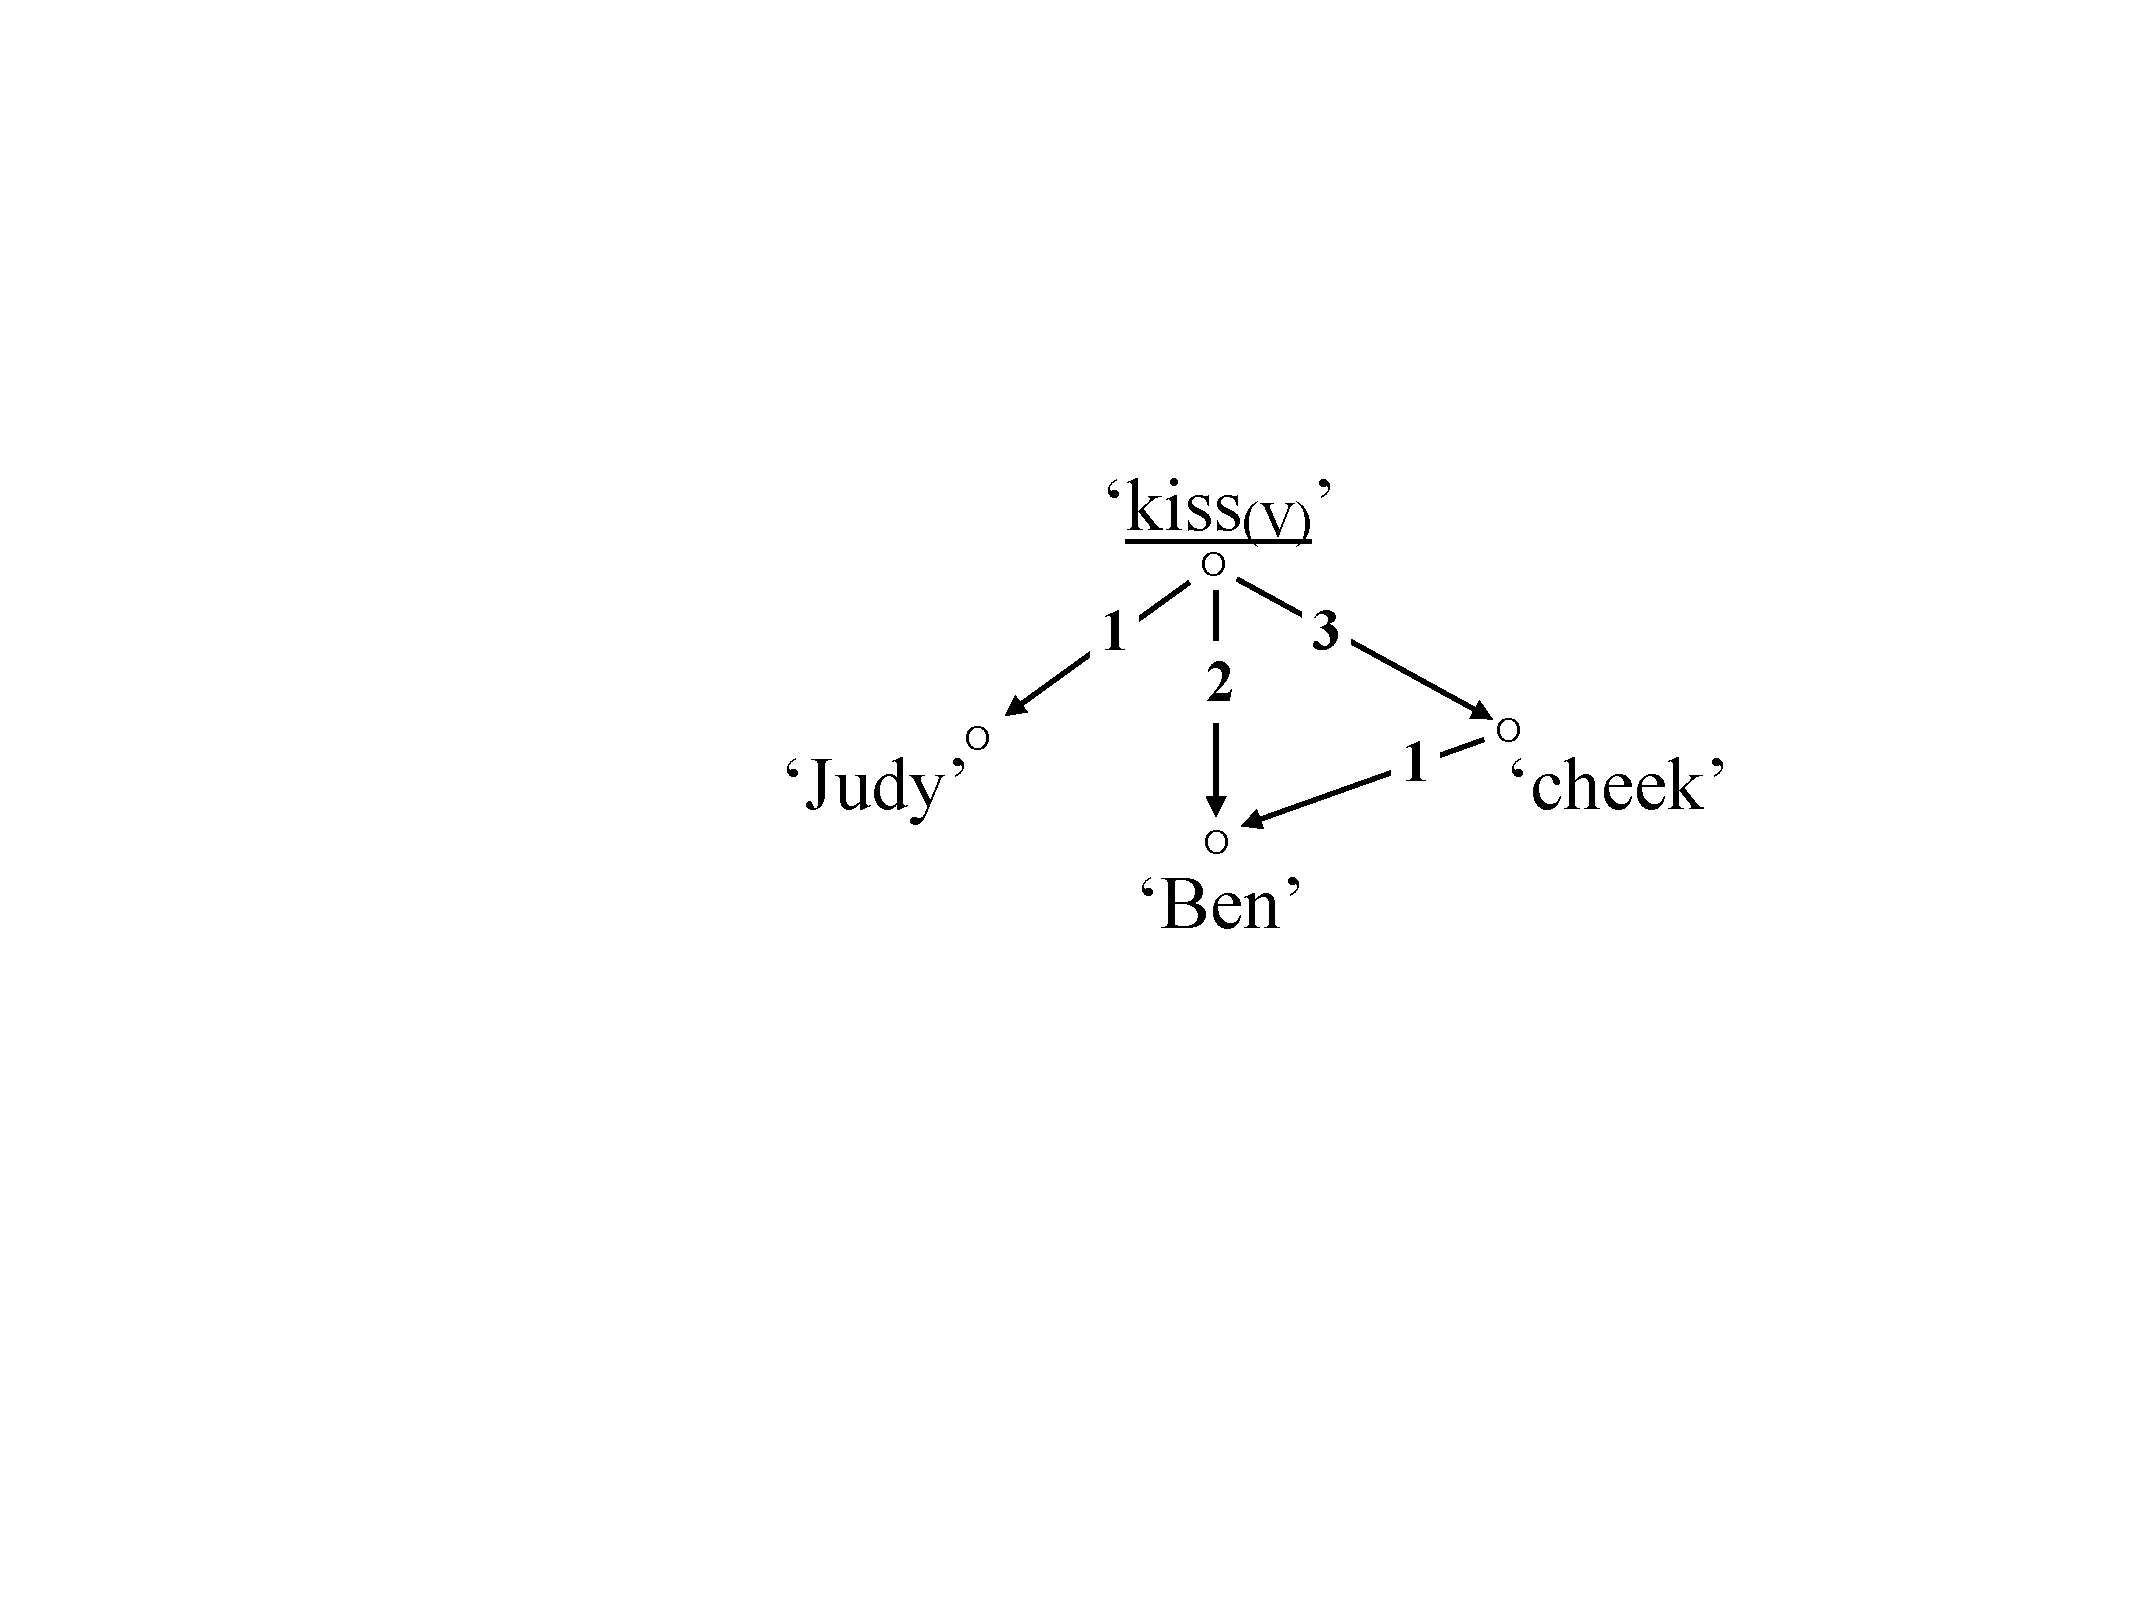
\includegraphics[width=4.5cm]{Fig/PrelimNotions/SemSJudyKissedBenCheek.pdf}
\caption{Semantic structure [SemS] of the sentence \textit{Judy kissed Ben on the cheek.}}\label{fig:SemSJudyKissedBenCheek}
\end{figure}

\noindent
The configuration of semantemes seen in \figref{fig:SemSJudyKissedBenCheek} is the \notion{semantic structure}\index[notion]{structure!semantic \tld\ [SemS]|emph}\index[notion]{semantic!\tld\ structure [SemS]|emph} [\notion{SemS}] of sentence \ref{ex:JudyKissedBenOnCheek} and of all its paraphrases\index[notion]{paraphrase}.\footnote{On paraphrasing, see \chapref{chap:NotionLF}, \sectref{sec:LFStandardParaphrasing} (p.\thinspace\pageref{sec:LFStandardParaphrasing}).} It calls for the following three comments.

\begin{quote}

\remark{Note.}The SemS in \figref{fig:SemSJudyKissedBenCheek} does not encode inflectional\index[notion]{inflection} meanings, that is, \notion{grammemes}\index[notion]{grammeme|emph} expressed in \ref{ex:JudyKissedBenOnCheek}: the indicative and the past tense of the verb \textsc{kiss}\tsub{(V)}, as well as the singular of the noun \textsc{cheek}. For simplicity's sake, we follow the same policy in all SemSs in this volume.

\end{quote}

\paragraph*{1) Communicatively dominant semanteme.}

The sentence \textit{Judy kissed Ben on the cheek} is about an act of kissing: therefore, the semanteme `\myuline{kiss}' is \notion{communicatively dominant}\index[notion]{communicative!\tld\ dominance|emph}, which is indicated by underscoring. By contrast, the noun phrase \textit{Ben's cheek that was kissed by Judy} is about the cheek (of Ben) and possesses an identical semantic structure, except for the semanteme `\myuline{cheek}', which is communicatively dominant (i.e., underscored in the semantic structure of this phrase).

Communicative dominance is an essential component of the \notion{communicative structure}\index[notion]{communicative!\tld\ structure|emph}\index[notion]{structure!communicative \tld|emph} of utterances, as theorized in \textcite{Polguere1990a-e} and \textcite{Melcuk2001b}. For the sake of simplicity, other components of communicative structures -- such as the Rheme\index[notion]{Rheme} vs. Theme\index[notion]{Theme} opposition -- are not encoded in utterance representations in this volume.

\paragraph*{2) Semantic actants' numbering.}

Numbering of SemAs of a predicative meaning depends on its internal structure, that is, on its semantic decomposition. Kissing someone is to act upon someone, and the Agent\index[notion]{Agent (semantic role)}\index[notion]{semantic!\tld\ role} of an action is taken to be SemA~\syntDname{1}, the Patient\index[notion]{Patient (semantic role)} undergoing an action is SemA~\syntDname{2}, and the Target\index[notion]{Target (semantic role)} of the kiss (part of the Patient's body) is SemA~\syntDname{3}.

\paragraph*{3) Semantic structure as a network.}

\figref{fig:SemSJudyKissedBenCheek} shows that the SemA~\syntDname{3} of `kiss' is a quasi-predicate that controls one actant slot: `cheek of X'. This is due to the fact that `cheek' is `part of the body of X [such that...]'; all names of body parts necessarily express quasi-predicative semantemes.  In this case, the SemA~\syntDname{1} of the quasi-predicate `cheek' is `Ben', and `Ben' is itself the SemA~\syntDname{2} of `kiss'. This configuration of semantic dependencies forms a \notion{semantic network}\index[notion]{semantic!\tld\ network|emph}\index[notion]{network \lfgp{see also \textit{graph}}!semantic \tld|emph}.

\begin{furtherreading}
On semantemes\index[notion]{semanteme}, see \textcite{MelcukPolguere2008}, \textcite{Polguere2012a} and \textcite[Part~II, Sec.~2.2, 193--205]{Melcuk2012a-e}; on communicative dominance\index[notion]{communicative!\tld\ dominance}, see \textcite[Part~I, Sec.~2.3.1.1]{Melcuk2001b}; on SemA numbering\index[notion]{actant!semantic \tld\ number}, see \textcite[Ch.~12, Sec.~3.4.2.3]{Melcuk2015a-e} and \textcite[Ch.~4, Sec.~3]{Melcuk2012a-e}; on Meaning-Text semantic networks, see \textcite{Polguere1997-e}.
\end{furtherreading}

\section{Syntactic notions}\label{sec:syntacticNotions}

From the viewpoint of syntactic structures, two levels of representation are distinguished, which can be approximately characterized as follows.

The \notion{deep-syntactic structure}\index[notion]{structure!deep-syntactic \tld\ [DSyntS]|emph}\index[notion]{deep-syntactic!\tld\ structure [DSyntS]|emph}\index[notion]{syntax!deep \tld|emph} [\notion{DSyntS}]\phantomsection\label{txt:DSyntS} is the most direct lexical and syntactic expression of the corresponding SemS. It contains only the semantically full lexical units of the sentence to be produced, connected by labeled \notion{deep-syntactic dependencies}\index[notion]{dependency!deep-syntactic \tld}, called \notion{deep-syntactic relations}\index[notion]{deep-syntactic!\tld\ relation}\index[notion]{relation!deep-syntactic \tld}. The resulting structure is a \notion{dependency tree}\index[notion]{dependency!\tld\ tree}\index[notion]{tree!dependency \tld}\index[notion]{tree!deep-syntactic \tld}\index[notion]{deep-syntactic!\tld\ tree}.

The \notion{surface-syntactic structure}\index[notion]{structure!surface-syntactic \tld\ [SSyntS]|emph}\index[notion]{surface-syntactic!\tld\ structure [SSyntS]|emph}\index[notion]{syntax!surface \tld|emph} [\notion{SSyntS}] is geared to the actual sentence in the sense that it serves to determine word order\index[notion]{word order} and morphological dependencies\index[notion]{dependency!morphological \tld}\index[notion]{morphology!morphological dependency} between lexemes, if any. It contains all and only the lexemes of the sentence to be produced, connected by labeled surface-syntactic dependencies, called \notion{surface-syntactic relations}\index[notion]{surface-syntactic!\tld\ relation}\index[notion]{relation!surface-syntactic \tld}. The resulting structure is, of course, also a dependency tree.

Let us illustrate the \notion{correspondences}\index[notion]{correspondence between representation levels|emph} between the SemS, the DSyntS and the SSyntS of a sentence, using sentence \Next as example.

\begingroup
\small

\ex. Judy shoots the breeze with Ben for hours.\label{ex:JudyShootsBreezeBenForHours}

\endgroup

``A\thinspace$\Leftrightarrow$\thinspace{}B'' means `linguistic entity A of the level $n$ of representation corresponds, i.e. is semantically equivalent, to linguistic entity B of level $n+1$; for instance, \figref{fig:sampleSemDSyntCorr} shows the SemS\thinspace$\Leftrightarrow$\thinspace{}DSyntS correspondence for \textit{Joey sleeps}.

\noindent
\begin{figure}

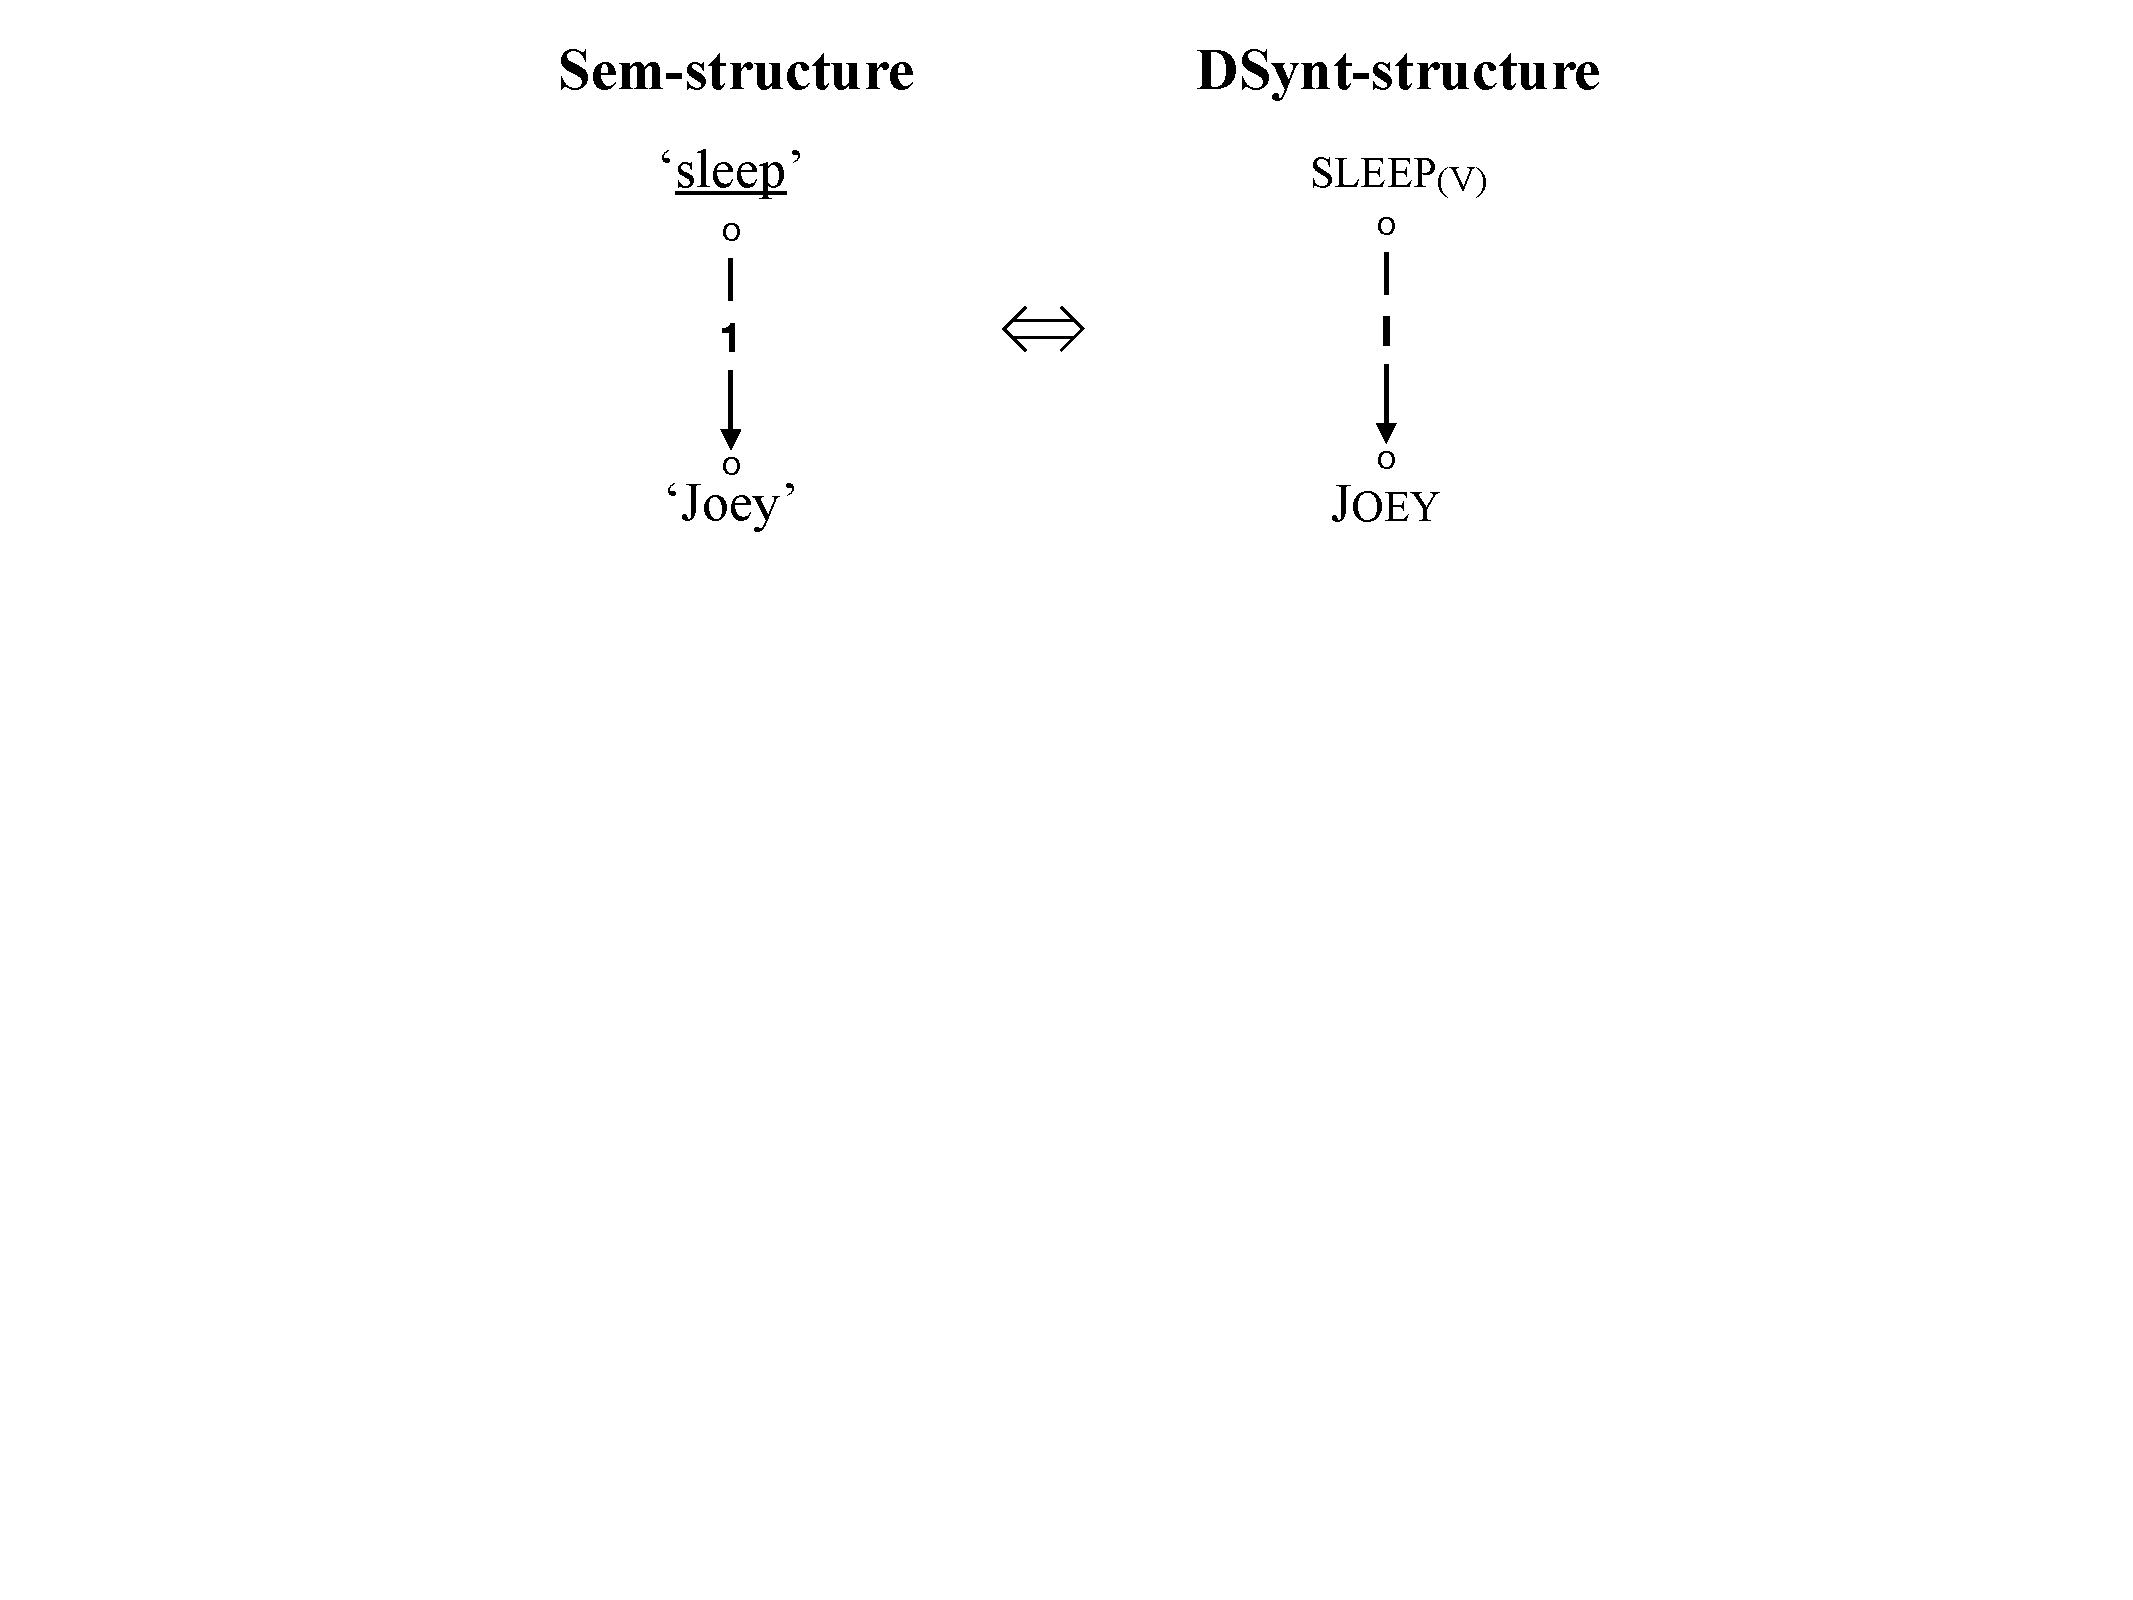
\includegraphics[width=6.5cm]{Fig/PrelimNotions/sampleSemDSyntCorr.pdf}
\caption{Example of a SemS\thinspace$\Leftrightarrow$\thinspace{}DSyntS correspondence}\label{fig:sampleSemDSyntCorr}
\end{figure}

In what follows we focus on  two particular correspondences between utterance structures: SemS\thinspace$\Leftrightarrow$\thinspace{}DSyntS and DSyntS\thinspace$\Leftrightarrow$\thinspace{}SSyntS.

\noindent
\begin{figure}

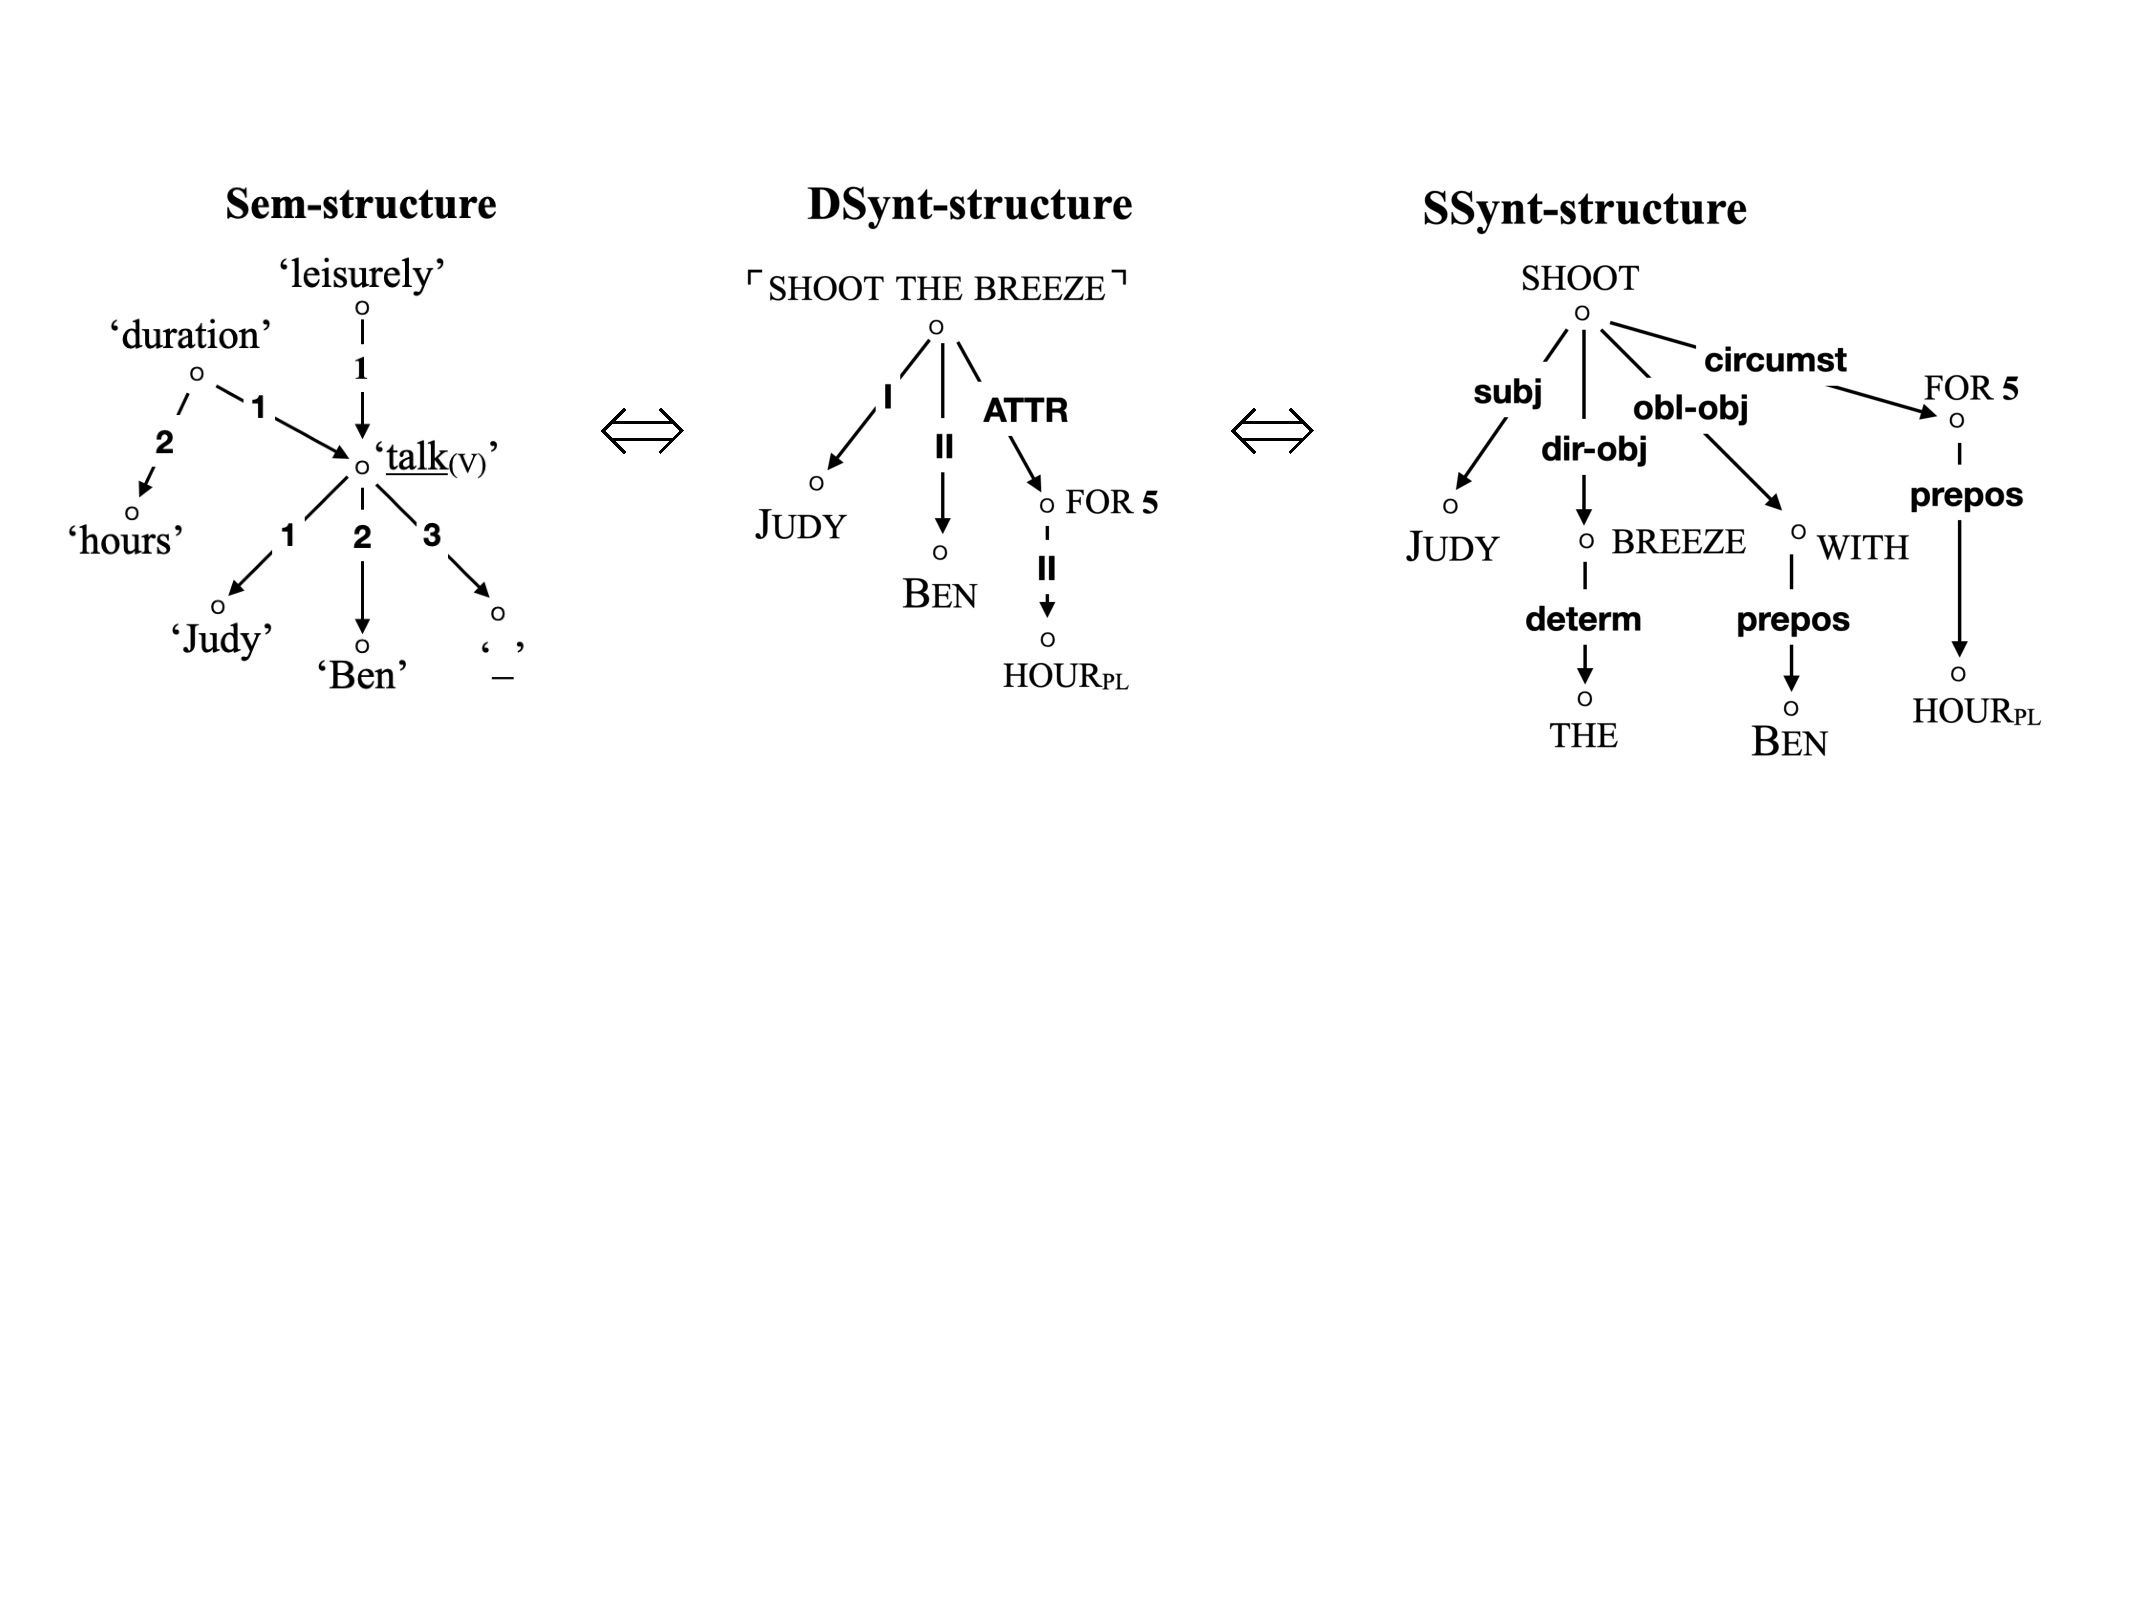
\includegraphics[width=\linewidth]{Fig/PrelimNotions/SemDSyntSSyntCorr.pdf}
\caption[SemS\thinspace$\Leftrightarrow$\thinspace{}DSyntS\thinspace$\Leftrightarrow$\thinspace{}SSyntS correspondences for the sentence\newline \textit{Judy shoots the breeze with Ben for hours.}]{SemS\thinspace$\Leftrightarrow$\thinspace{}DSyntS\thinspace$\Leftrightarrow$\thinspace{}SSyntS correspondences for sentence \ref{ex:JudyShootsBreezeBenForHours}: \textit{Judy shoots the breeze with Ben for hours.}}\label{fig:SemDSyntSSyntCorr}
\end{figure}

The SemS\index[notion]{semantic!\tld\ structure [SemS]}\index[notion]{structure!semantic \tld\ [SemS]} has been introduced and explained in \sectref{sec:semanticNotions}. Here we need to explain the DSyntS and the SSyntS.

\paragraph*{Deep-syntactic structure [DSyntS] of sentence \ref{ex:JudyShootsBreezeBenForHours}.}\index[notion]{deep-syntactic!\tld\ structure [DSyntS]}\index[notion]{structure!deep-syntactic \tld\ [DSyntS]}

The nodes of this tree\index[notion]{tree!deep-syntactic \tld|emph}\index[notion]{deep-syntactic!\tld\ tree|emph} are labeled with \notion{deep lexical units}\index[notion]{lexical unit!deep \tld|emph}, i.e., semantically full lexical units, which express semantemes of the SemS. The idiom \idiom{\textsc{shoot the breeze}} expresses the semantic configuration `leisurely\thinspace\syntRel{1}\thinspace\myuline{talk}\tsub{(V)}', and the meaningful preposition\index[notion]{preposition} \textsc{for}\sensenum{5}, the semanteme `duration'.\footnote{The lexicographic number of \textsc{for}\sensenum{5} comes from the online \textit{Longman Dictionary of Contemporary English} \parencite{Longman2025}, henceforth LDOCE.}\index[notion]{dictionary!Longman Dictionary of Contemporary English@\textit{Longman Dictionary of Contemporary English} [LDOCE]}\index[notion]{Longman Dictionary of Contemporary English@\textit{Longman Dictionary of Contemporary English} [LDOCE]}\index[notion]{lexicographic number} The other nodes are self-explanatory.

The arcs (branches) of this tree are labeled with DSynt-relations of two types:

\begin{itemize}

\item \syntDname{I} and \syntDname{II} are \notion{actantial DSynt-relations}\index[notion]{actantial relation|emph}\index[notion]{relation!actantial \tld|emph}: the dependent\index[notion]{dependent, syntactic} members of these relations -- \textsc{Judy} and \textsc{Ben} -- are DSynt-actants\index[notion]{actant!deep-syntactic \tld\ [DSyntA]}\index[notion]{deep-syntactic!\tld\ actant [DSyntA]} of their governor, the idiom \idiom{\textsc{shoot the breeze}} (`X \idiom{shoots the breeze} with Y'). The notion of DSynt-actant will be defined shortly (p.\thinspace\pageref{def:DSyntA}).

\item \syntDname{ATTR}\index[notion]{ATTR@\syntDname{ATTR}|emph}\phantomsection\label{txt:ATTRDSyntR} is a non-actantial DSynt-relation: it is not foreseen by the meaning of its governor\index[notion]{governor, syntactic} and represents a dependency inversion -- called \notion{head-switching}\index[notion]{head-switching} -- with respect to the corresponding semantic relation; cf.~\figref{fig:SDSyntSDependencyInversion}.

\end{itemize}

\begin{figure}

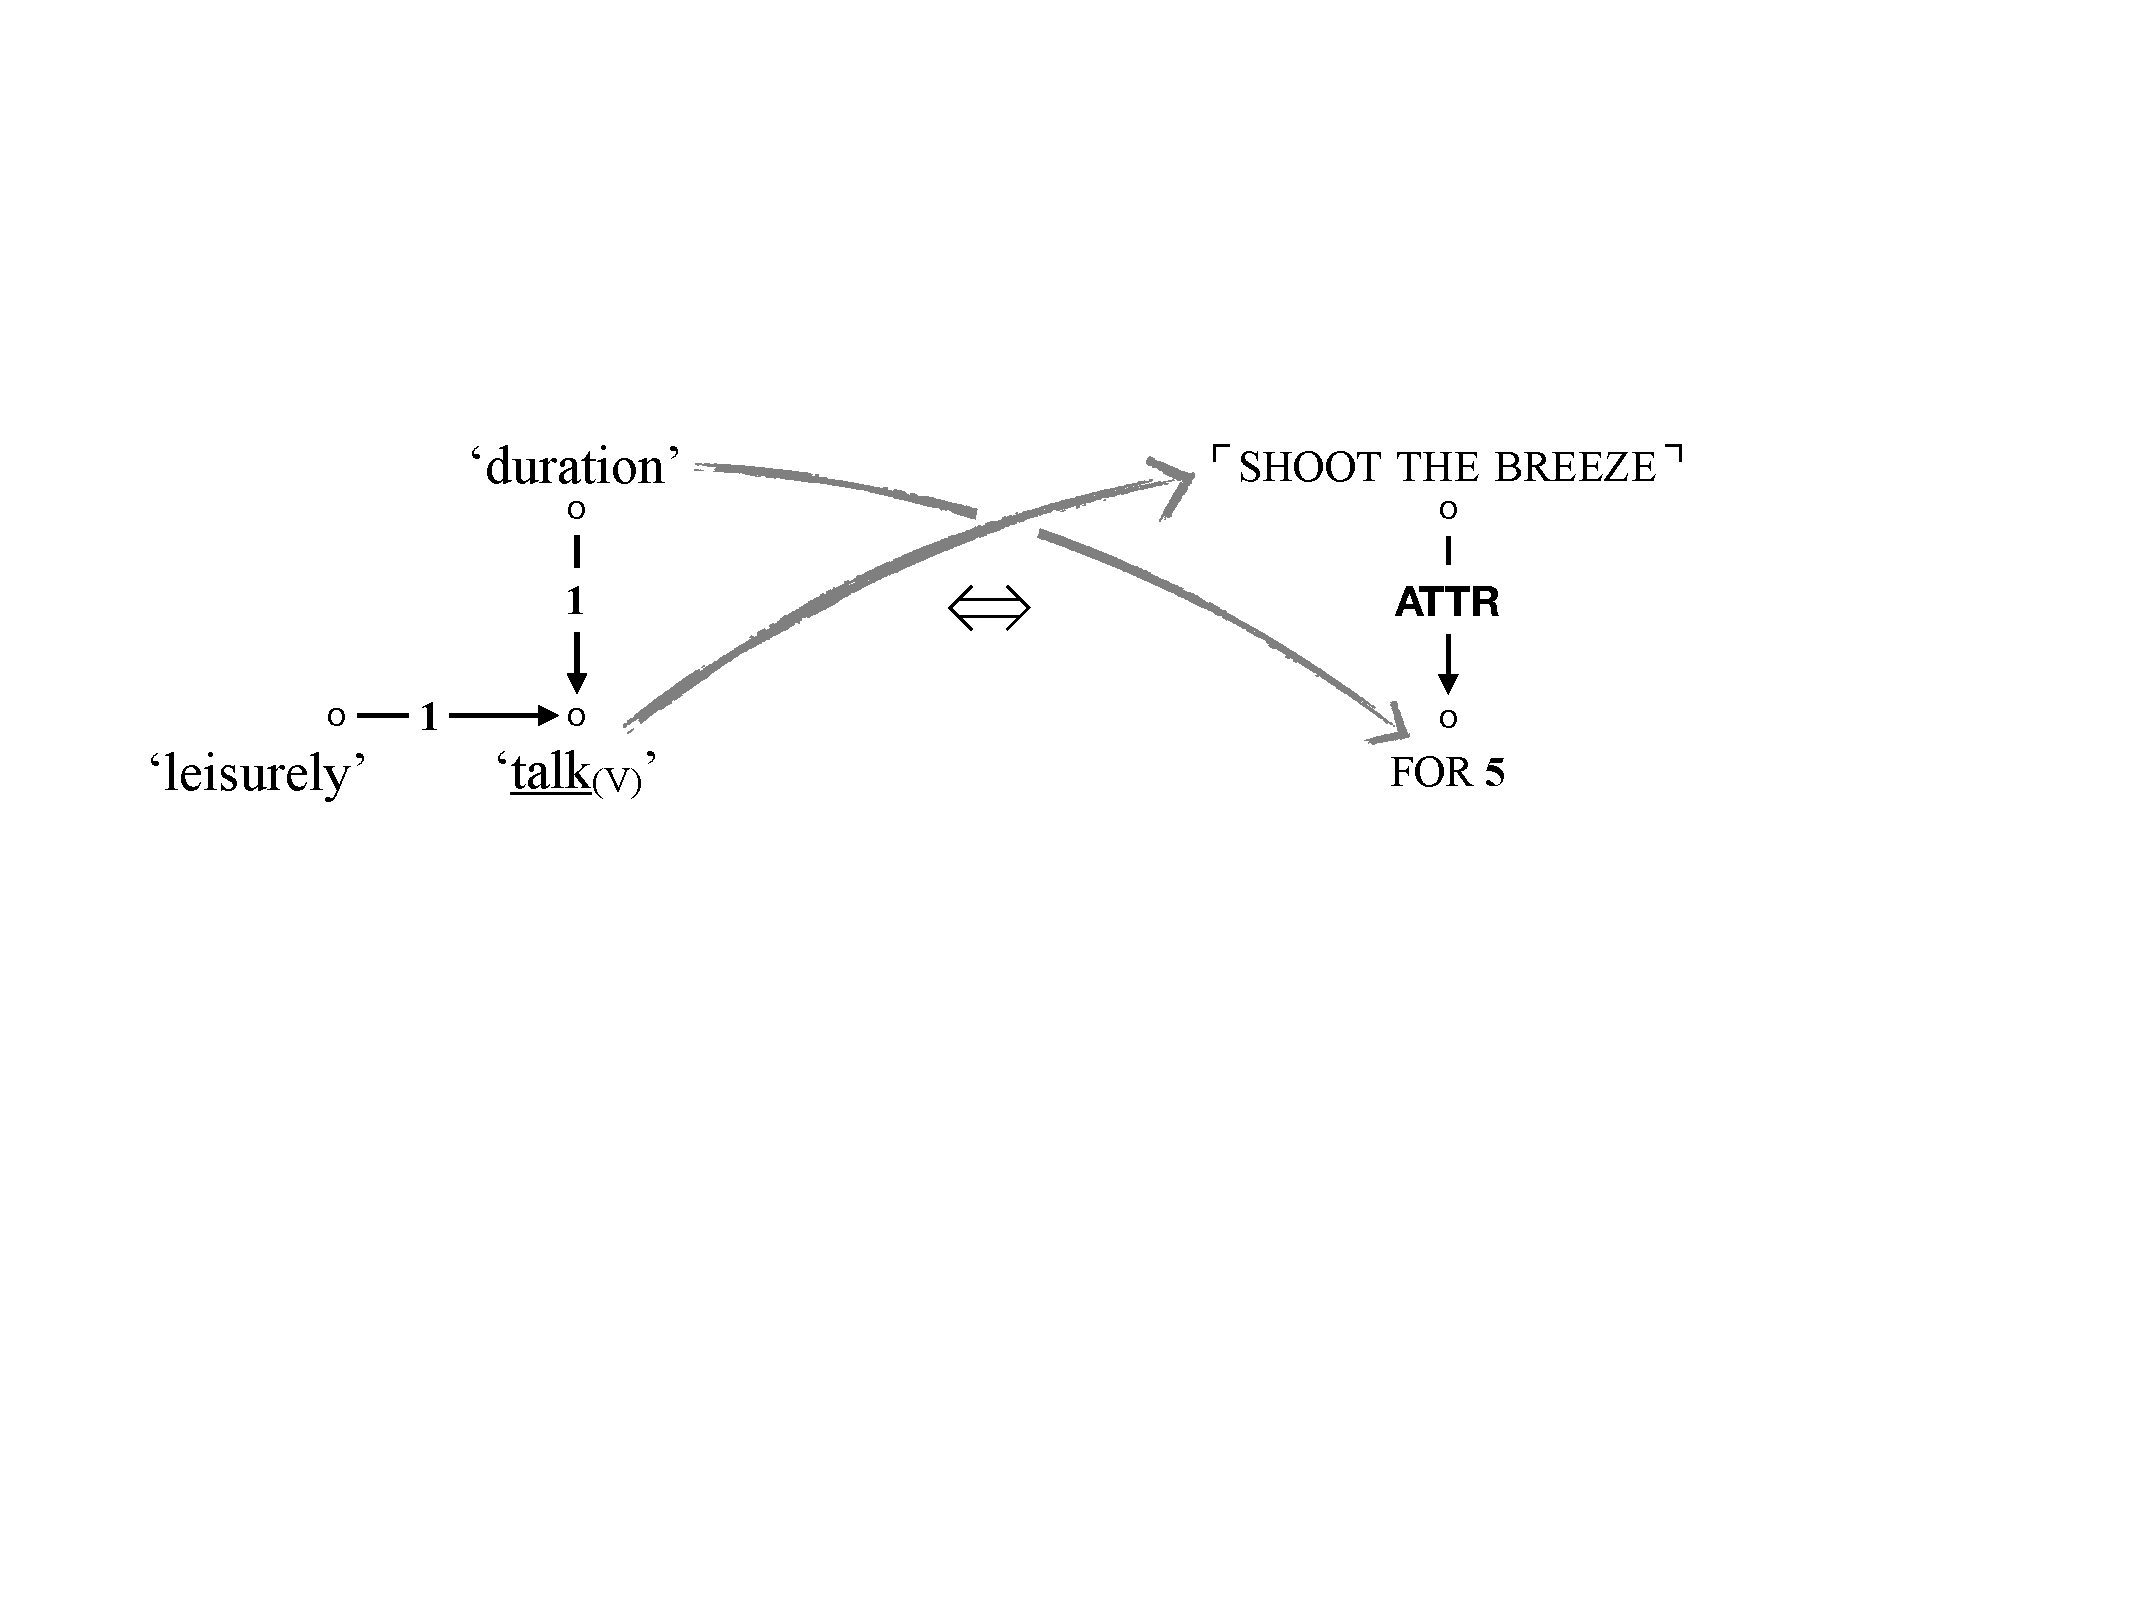
\includegraphics[width=10.5cm]{Fig/PrelimNotions/SemSDSyntSDependencyInversion.pdf}
\caption[SemS\thinspace$\Leftrightarrow$\thinspace{}DSyntS dependency inversion \[=~head-switching\]\newline involving the DSynt-relation \syntDname{ATTR}]{SemS\thinspace$\Leftrightarrow$\thinspace{}DSyntS dependency inversion [=~head-switching] involving the \mbox{DSynt-relation} \syntDname{ATTR}}\label{fig:SDSyntSDependencyInversion}
\end{figure}

At the DSynt-level several other DSynt-relations are used -- they are listed below. These relations are language-universal\index[notion]{language-universal}. In the present volume only actantial and \syntDname{ATTR}(ibutive) DSynt-relations are relevant.

\phantomsection\label{tab:listDSyntRels}\begin{soundbox}{Language-universal DSynt-relations}
\vspace{-14pt}
\small
\setlength{\tabcolsep}{3pt}
\setlength\extrarowheight{1pt}
\begin{longtable}{ l >{\raggedright\arraybackslash}p{8.8cm} }

\syntDname{I} & 1\tsup{st} deep-syntactic relation\slashs1\tsup{st} deep-syntactic actant \\*
\syntDname{II} & 2\tsup{nd} deep-syntactic relation\slashs2\tsup{nd} deep-syntactic actant [\textit{Joey}\thinspace\syntRelLeft{I}\thinspace\textit{loves}\thinspace\syntRel{II}\thinspace\textit{food}] \\*
\syntDname{...} & \\[+3pt]

\syntDname{APPEND} & appenditive; it links an structurally extraneous element, such as a parenthetical or an interjection\index[notion]{interjection}, to its governor\index[notion]{governor, syntactic} -- the syntactic head of the clause [\textit{Sorry,}\thinspace\syntRelLeft{APPEND}\syntRelChunk{{\relsize{-1.5}[\textit{I}]}}\thinspace\textit{am late}] \\

\syntDname{ADDRESS} & addressative; it links a direct address to its governor, which is the syntactic head of the clause [\textit{Yes,}\thinspace\syntRel{ADDRESS}\thinspace\textit{Sir}] \\

\syntDname{ATTR} & attributive; it links a restrictive modifier\slashs{}circumstantial to its governor [\textit{curious}\thinspace\syntRelLeft{ATTR}\thinspace\textit{student}; \textit{arrived}\thinspace\syntRel{ATTR}\thinspace\textit{yesterday}] \\

\syntDname{ATTR\tsub{qual}} & qualificative attributive; it links a qualificative modifier\thinspace/ circumstantial to its governor [\textit{students,}\thinspace \syntRel{ATTR\tsub{qual}}\thinspace\textit{hungry for knowledge}] \\

\syntDname{COORD} & coordinative; it links the dependent\index[notion]{dependent, syntactic} member of a syntactic coordination to its governor [\textit{Ben}\thinspace\syntRel{COORD}\thinspace\textit{and Judy}] \\

\syntDname{PSEUDO-COORD} & pseudo-coordinative; it links the dependent member of elaboration or clarification to its governor \\*
& [\textit{She came last year,}\thinspace\syntRel{PSEUDO-COORD}\thinspace\textit{in the spring}] \\

\end{longtable}
\end{soundbox}\index[notion]{circumstantial}

A notion playing a key role in the presentation of lexical functions is that of \notion{deep-syntactic actant}\index[notion]{actant!deep-syntactic \tld\ [DSyntA]|emph}\index[notion]{deep-syntactic!\tld\ actant [DSyntA]|emph} [\notion{DSyntA}]\index[notion]{DSyntA [deep-syntactic actant]|see{actant (deep-syntactic)}}, mentioned above. It is defined as follows.

\begin{notiondefinition}{deep-syntactic actant [DSyntA]}
\phantomsection\label{def:DSyntA}A \notion{deep-syntactic actant} \syntDname{I}, \syntDname{II}, ... of lexical unit L is a DSynt-dependent\index[notion]{dependent, syntactic} of L such that\vspace{3pt} \\*
\setlength{\tabcolsep}{.5pt}\begin{tabular}{ p{0.2cm} >{\raggedright\arraybackslash}p{11cm} }
\SpecDiff & it expresses, in a prototypical case, a SemA of L and it is governed by L via an actantial DSynt-relation \syntDname{I}, \syntDname{II}, ... \\
\end{tabular}
\end{notiondefinition}

There is also a frequent enough possibility of a DSyntA of L coming, or being raised, to L from one of its DSyntAs. Such \notion{syntactic raising}\index[notion]{raising, syntactic} is illustrated in \figref{fig:DSyntARaising}. This figure presents one of the support verbs\index[notion]{support verb}\index[notion]{verb!support \tld} mentioned in \chapref{chap:Introduction} (\sectref{sec:aboutWhat}), namely the lexical function \lf{Oper\tsub{1}}\index[lf]{Operi@\lf{Oper\tsub{i}}!\lf{Oper\tsub{1}}} (\chapref{chap:syntLFs}, [\ref{lf:Oper-i}], p.\thinspace\pageref{lf:Oper-i}).

\lfappl{Oper\tsub{1}}{\textit{attack}\tsub{(N)}} is expressed in the surface-syntactic structure\index[notion]{surface-syntactic!\tld\ structure [SSyntS]}\index[notion]{structure!surface-syntactic \tld\ [SSyntS]} (see SSyntS below) by the lexical units \idiom{\textsc{carry out}} or \textsc{conduct}\tsub{(V)}. The \notion{actant transfer}\index[notion]{actant!transfer of deep-syntactic \tld} illustrated in \figref{fig:DSyntARaising} is common with verbal syntagmatic lexical functions (support and realization verbs) -- see \chapref{chap:syntLFs}, ``\nameref*{par:transferOfLsActants},'' p.\thinspace\pageref{par:transferOfLsActants}.

\begin{quote}
\remark{Remark.}\phantomsection\label{remark:raising}The second sentence (with raising) in \figref{fig:DSyntARaising} is dubious: speakers seem to accept it only with a special prosody, namely, pauses before and after \textit{on the fort}: \textit{The enemy carried out -- on the fort -- a massive attack}. Other languages, such as French and Russian, allow for this construction without problem, as shown in \Next[a-b].
\end{quote}

\begingroup
\small

\ex. \a. {\smaller French} L'ennemi a mené contre le fort une attaque massive.
     \b. {\smaller Russian} Vrag provël na fort massirovannuju ataku.

\endgroup

\begin{figure}
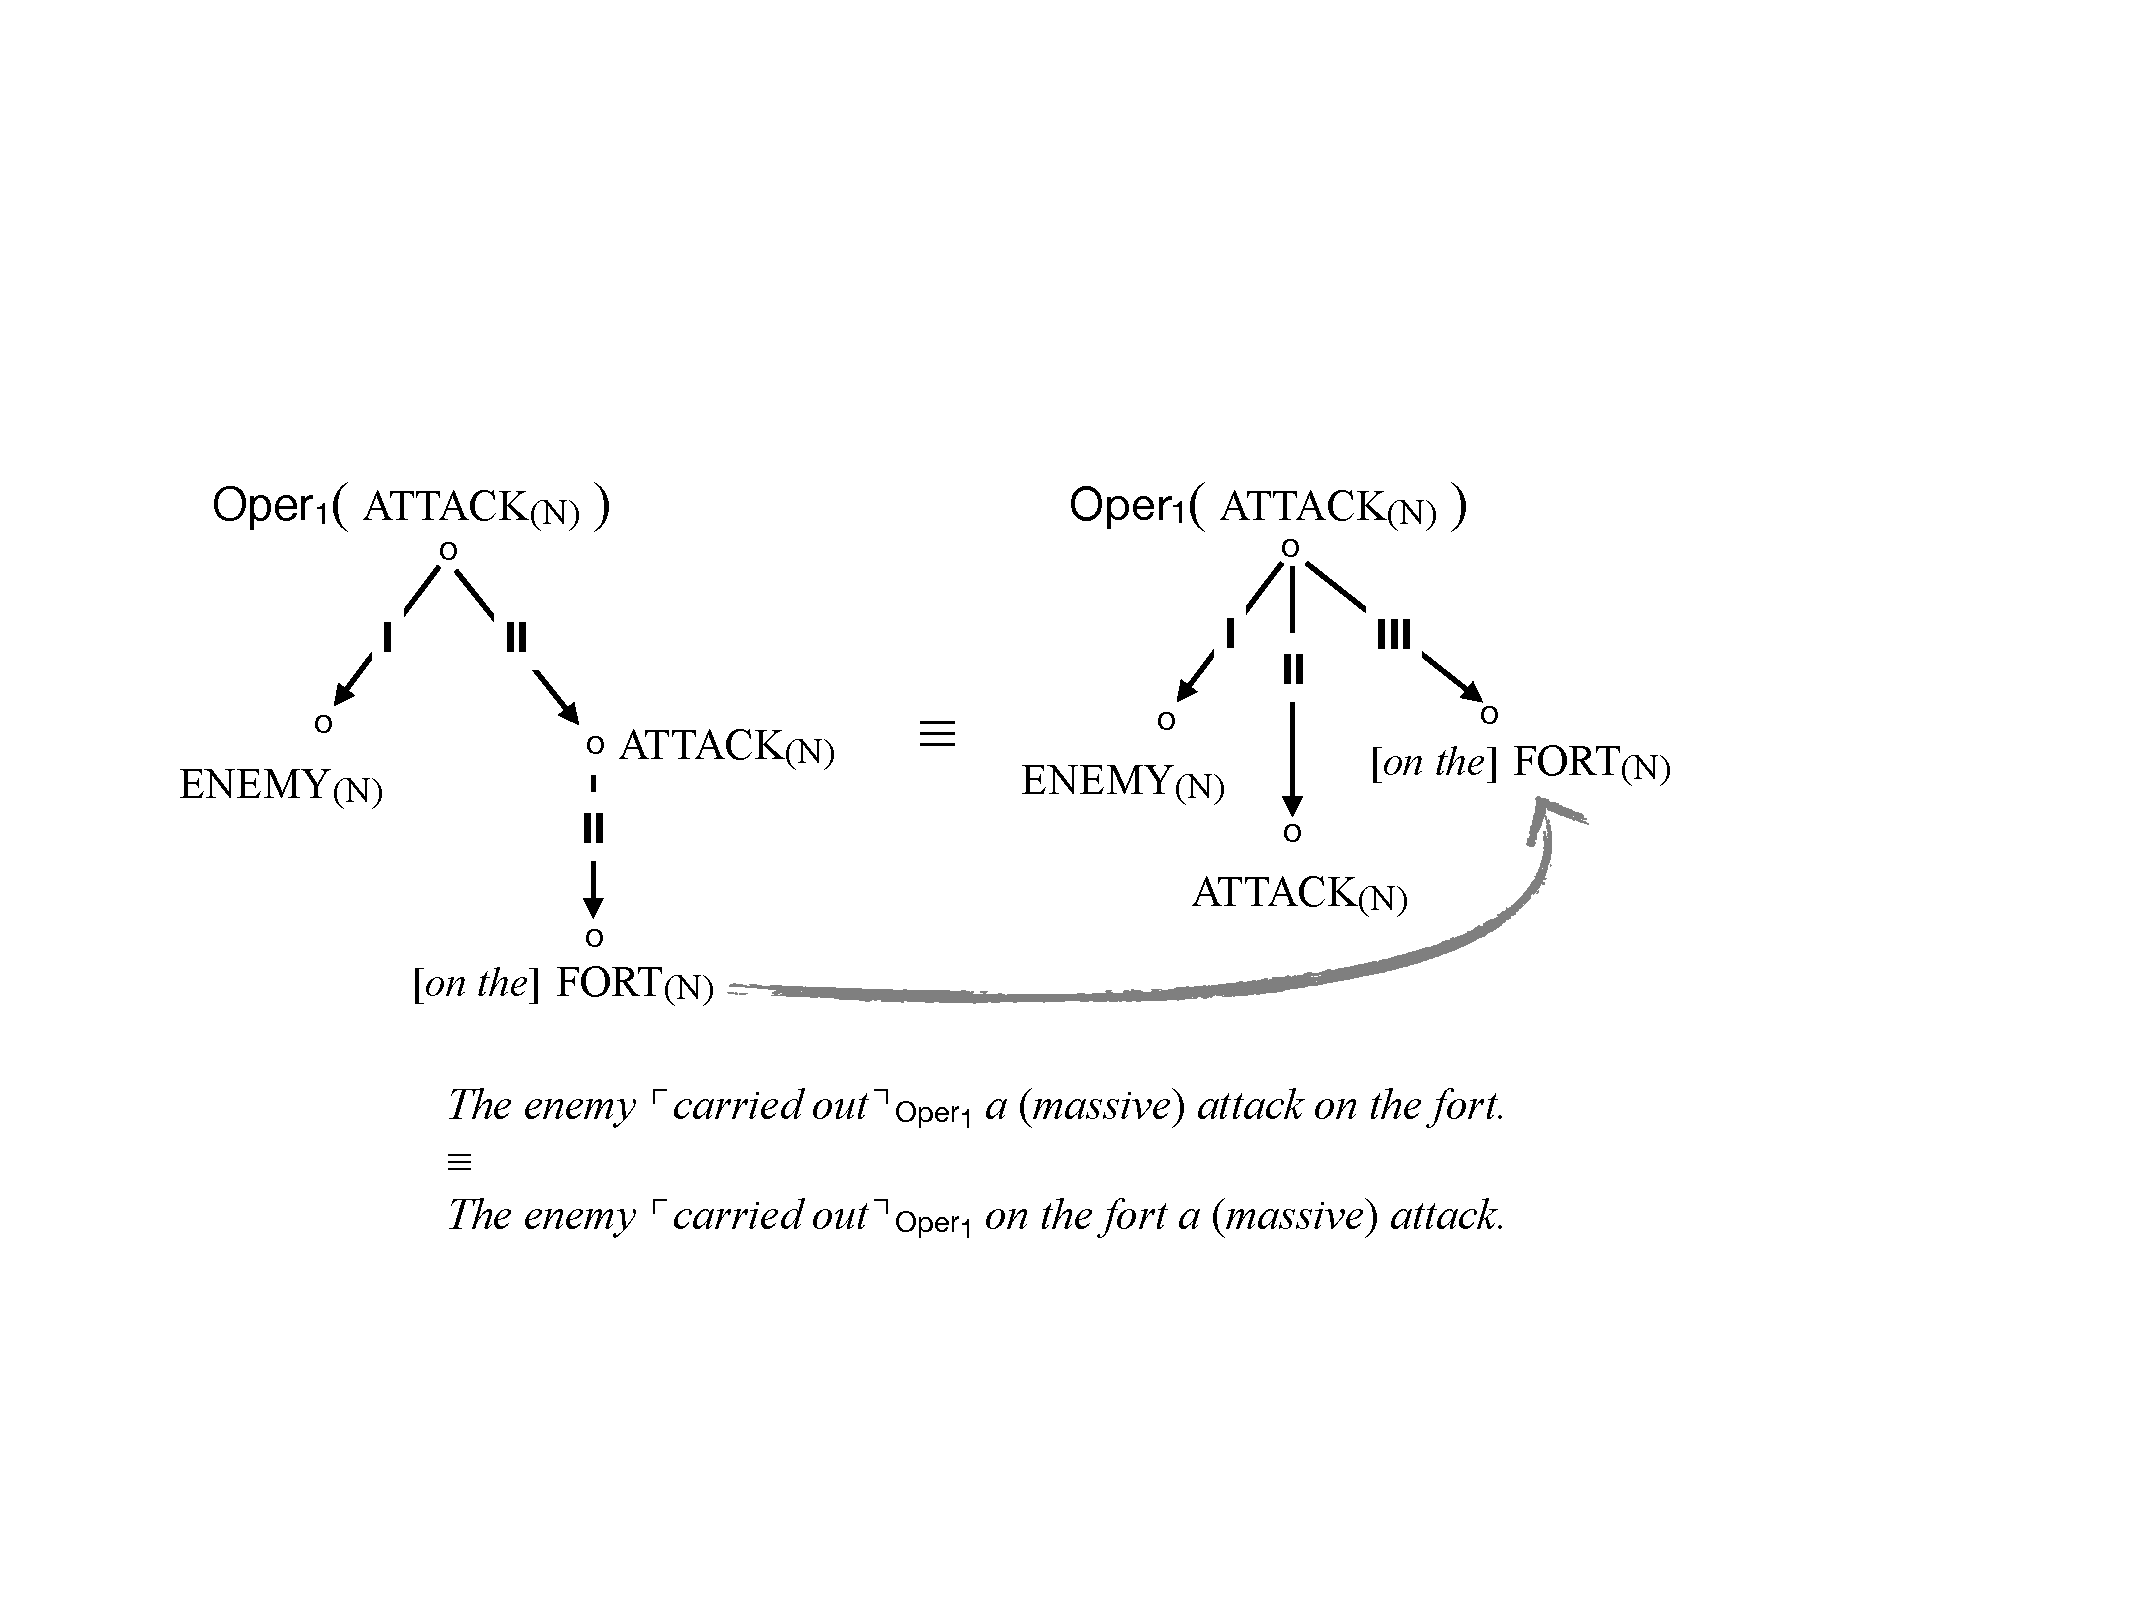
\includegraphics[width=11cm]{Fig/PrelimNotions/DSyntARaising.pdf}
\caption{Syntactic raising of a DSyntA}\label{fig:DSyntARaising}
\end{figure}

\paragraph*{Surface-syntactic structure [SSyntS] of sentence \ref{ex:JudyShootsBreezeBenForHours}.}\index[notion]{surface-syntactic!\tld\ structure [SSyntS]}\index[notion]{structure!surface-syntactic \tld\ [SSyntS]}

The nodes of the SSynt-tree\index[notion]{tree!surface-syntactic \tld|emph}\index[notion]{surface-syntactic!\tld\ tree} for \ref{ex:JudyShootsBreezeBenForHours} are labeled with all lexemes of the sentence, including lexical components of the idiom (\textsc{shoot}, \textsc{breeze} and \textsc{the}) and a governed preposition\index[notion]{preposition} (\textsc{with}).

The arcs of this tree are labeled with SSynt-relations\index[notion]{surface-syntactic!\tld\ relation}, which are language-specific -- i.e., non-universal\index[notion]{language-universal}; there are several dozens of SSynt-relations in a language. We list below SSynt-relations featured in \figref{fig:SemDSyntSSyntCorr} (p.\thinspace\pageref{fig:SemDSyntSSyntCorr}) and in the whole volume.

\phantomsection\label{tab:listSSyntRels}\begin{soundbox}{Some SSynt-relations of English}
\vspace{-14pt}
\small
\setlength{\tabcolsep}{2.2pt}
\setlength\extrarowheight{1pt}
\begin{longtable}{ l >{\raggedright\arraybackslash}p{8.3cm} }

\syntDname{circumstantial} &  \textit{talked}\thinspace\syntRel{circumst}\thinspace\textit{for} {\relsize{-1.5}[\textit{hours}]} \\
\syntDname{determinative} &  \textit{the}\thinspace\syntRelLeft{determ}\thinspace\textit{breeze}; \textit{my}\thinspace\syntRelLeft{determ}\thinspace\textit{daughter} \\
\syntDname{direct-objectival} &  \textit{shoot}\thinspace\syntRel{dir-obj}\thinspace\textit{breeze}; \textit{Marry}\thinspace\syntRel{dir-obj}\thinspace\textit{me};\newline \textit{want}\thinspace\syntRel{dir-obj}\thinspace\textit{to} {\relsize{-1.5}[\textit{go}]}; \textit{declare}\thinspace\syntRel{dir-obj}\thinspace\textit{that} {\relsize{-1.5}[\textit{it's OK}]} \\
\syntDname{modificative} &  \textit{big}\thinspace\syntRelLeft{modif}\thinspace\textit{deal} \\
\syntDname{oblique-objectival} &  \textit{shoot} {\relsize{-1.5}[\textit{breeze}]}\thinspace\syntRel{obl-obj}\thinspace\textit{with} {\relsize{-1.5}[\textit{Ben}]}; \textit{rely}\thinspace\syntRel{obl-obj}\thinspace\textit{on} {\relsize{-1.5}[\textit{you}]} \\
\syntDname{possessive} &  \textit{tomorrow's}\thinspace\syntRelLeft{possess}\thinspace\textit{event} \\
\syntDname{prepositional} &  \textit{with}\thinspace\syntRel{prepos}\thinspace\textit{Ben}; \textit{for}\thinspace\syntRel{prepos}\thinspace\textit{hours} \\
\syntDname{subjectival} &  \textit{Judy}\thinspace\syntRelLeft{subj}\thinspace\textit{shoots} {\relsize{-1.5}[\textit{the breeze}]}; \textit{it}\thinspace\syntRelLeft{subj}\thinspace\textit{is} {\relsize{-1.5}[\textit{late}]} \\
\syntDname{subjectival-adnominal} &  \textit{speech}\thinspace\syntRel{subj-adnom}\thinspace\textit{of} {\relsize{-1.5}[\textit{the President}]} \\

\end{longtable}
\end{soundbox}\index[notion]{object, syntactic!direct \tld}\index[notion]{object, syntactic!oblique \tld}\index[notion]{subject, syntactic}\index[notion]{circumstantial}

\largerpage[-1]
\paragraph*{Active syntactic valence.}\label{para:activeSyntacticValence}

SemS\thinspace$\Leftrightarrow$\thinspace{}DSyntS\thinspace$\Leftrightarrow$\thinspace{}SSyntS correspondences\index[notion]{correspondence between representation levels} are essentially based on the actantial structures -- i.e., sets of actants -- of lexical units. More precisely, these correspondences are controlled by the \notion{active syntactic valence}\index[notion]{valence!active syntactic \tld|emph} of each lexical unit L they involve: how L's SemAs are expressed by means of DSyntAs, and how the latter are expressed at the surface-syntactic and morphological levels\index[notion]{morphology}.\footnote{Unlike the situation with semantic valence (cf. \sectref{sec:semanticNotions}, p.\thinspace\pageref{par:semanticValence} above), the adjective \textit{active} is required since active syntactic valence contrasts with passive syntactic valence: see \chapref{chap:NotionLF}, \sectref{sec:notionPdD}.}\index[notion]{valence!semantic \tld}\index[notion]{valence!passive syntactic \tld}

Consequently, to implement SemS\thinspace$\Leftrightarrow$\thinspace{}DSyntS\thinspace$\Leftrightarrow$\thinspace{}SSyntS correspondences, the information about active syntactic valence of lexical units is needed. It is specified in their lexical entries\index[notion]{lexical entry} by means of a table, called the \notion{government pattern}\index[notion]{government pattern|emph}\phantomsection\label{txt:governmentPattern}. As an illustration, we give in \ref{ex:GPofKISS-v} the government pattern of the verb \textsc{kiss}\tsub{(V)}, appearing earlier in sentence \ref{ex:JudyKissedBenOnCheek} -- \sectref{sec:semanticNotions}, p.\thinspace\pageref{ex:JudyKissedBenOnCheek}.\footnote{A lexical unit may have more than one government pattern. Thus, \textsc{kiss}\tsub{(V)} has another government pattern that describes utterances where the verb's SemA\thinspace\syntDname{3} (`Z') is expressed as its direct object (cf. \textit{Judy kissed Ben's cheek}):\medskip\\
\hphantom{.......}\begin{tabular}{ >{\raggedright\arraybackslash}p{1.6cm} >{\raggedright\arraybackslash}p{2cm} }
\midrule
\multicolumn{1}{c}{`X'~$\Leftrightarrow$~\textsf{\textbf{I}}}
& \multicolumn{1}{c}{`Z'~$\Leftrightarrow$~\textsf{\textbf{II}}} \\
\midrule
{\small 1.} \syntRel{subj}\thinspace N
& {\small 1.} \syntRel{dir-obj}\thinspace N \\
\midrule
\end{tabular}}\index[notion]{object, syntactic!direct \tld}

\ex.\label{ex:GPofKISS-v} \begin{tabular}{ >{\raggedright\arraybackslash}p{1.9cm} >{\raggedright\arraybackslash}p{2.2cm} >{\raggedright\arraybackslash}p{2.7cm} }
\midrule
\multicolumn{1}{c}{`X'~$\Leftrightarrow$~\textsf{\textbf{I}}}
& \multicolumn{1}{c}{`Y'~$\Leftrightarrow$~\textsf{\textbf{II}}}
& \multicolumn{1}{c}{`Z'~$\Leftrightarrow$~\textsf{\textbf{III}}} \\
\midrule
{\small 1.} \syntRel{subj}\thinspace N
& {\small 1.} \syntRel{dir-obj}\thinspace N
& {\small 1.} \syntRel{obl-obj}\thinspace \textit{on} N \\
\midrule
\end{tabular}

Another example of government pattern, for the noun \textsc{anger}\tsub{(N)}, is found in the Appendix, p.\thinspace\pageref{fig:governmentPatternANGER-n}.

The government pattern of a given lexical unit L describes L's restricted \emph{syntactic} cooccurrence\index[notion]{cooccurrence, restricted!syntactic \tld} in L's lexical entry\index[notion]{lexical entry}. By contrast, lexical functions\index[notion]{lexical function} -- the topic of the present volume -- describe restricted \emph{lexical} cooccurrence\index[notion]{cooccurrence, restricted!lexical \tld} of lexical units.

\begin{furtherreading}
On the notion of DSyntA, see \textcite[Ch.~12]{Melcuk2015a-e}; on the correspondence between the SemS and the DSyntS, see \textcite{Polguere1990a-e} and \textcite[Ch.~10]{Melcuk2013c-e}; on SSynt-relations, see \textcites{Melcuk2015c}{Melcuk2016b}[Ch.~2]{Melcuk2021a}; on government patterns, see \textcite{Milicevic2009a} and \textcite[Ch.~13]{Melcuk2015a-e}.
\end{furtherreading}

\clearpage{\pagestyle{empty}\cleardoublepage}

